%%%%%%%%%%%%%%%%%%%%%%%%%%%%%%%%%%%%%%%%%%%%%%%%%%%%%%%%%%%%%%%%%%%%%%%%%
% CHAPTER Theory
%%%%%%%%%%%%%%%%%%%%%%%%%%%%%%%%%%%%%%%%%%%%%%%%%%%%%%%%%%%%%%%%%%%%%%%%%

\chapter[Theory]{Theory}
\label{cha:theory}

\minitoc

% \input{}



%%%%%%%%%%%%
%%from HPCA
%%background
% In Figure~\ref{fig:banded_mat_def}, we illustrate a banded, square matrix of dimension $M$.
% We define $w_B$ as the width of the banded region, or \textit{bandwidth}, as shown in \textit{red} in the figure. 
% Sometimes it is easier to refer to the half-\textit{bandwidth}, $w_{hB}$, which respects the relation $w_B = 2w_\mathit{hB} - 1$.
% The average density in the band and out of the band is defined as $d_\mathit{IB}$ and $d_\mathit{OB}$, respectively.
% In a \textit{perfectly banded} matrix, there are no elements outside the band, thus $d_\mathit{OB} = 0$.

% \begin{figure}[htbp]
%     \centering
%     % \begin{minipage}[b]{0.33980583\linewidth} % 17.5/51.5
%     %     \begin{figure}[H]
%     %         \centering
%     %         
\includegraphics[width=\linewidth]{Figures/PDF/MatrixDef.pdf}
%     %         \caption{Banded Matrix Definition}
%     %         \label{fig:banded_mat_def}
%     %     \end{figure} 
%     % \end{minipage}
%     % \hfill
%     \begin{minipage}[b]{0.63106796\linewidth} % 32.5/51.5
%         \begin{figure}[H]
%             \centering
%             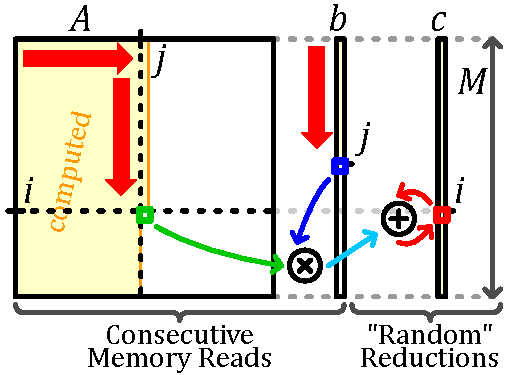
\includegraphics[width=\linewidth]{Figures/PDF/MatrixSpMVRep.pdf}
%             \caption{Visual Representation of \algo{OP} SpMV Computation}
%             \label{fig:op_spmv_rep}
%         \end{figure}
%     \end{minipage}
% \end{figure}

% Sparse matrices are used in many kernels, such as sparse matrix-vector (SpMV) and sparse matrix-matrix multiplication (SpMM).
% These kernels can be implemented with several algorithms.
% Many works~\cite{Isaac2024_SoA, Mukkara2019_PHI, Pal2018_OuterSPACE} have shown that the \textit{Outer-Product} (\algo{OP}) algorithm has the potential to enhance performance, if computed with an adapted hardware architecture.
% For sparse kernels, the performance is almost always limited by the indirect accesses induced by the sparse formats.
% The indirections are ``random'' and have limited spatial and temporal locality, limiting the effectiveness of traditional caches.
% For \algo{OP} algorithms, these indirect accesses occur when updating the output vector, which are referred to as ``scatter updates''.

% Many software solutions focus on improving performance, using conventional compute hardware including CPUs and GPUs~\cite{MOHAMMED_2022_SPARSE}, but since the performance limitation comes from the memory system, custom hardware solutions are required.
% PHI~\cite{Mukkara2019_PHI}, SortCache~\cite{Srikanth2021_SortCache} and ASA~\cite{Zhang2022_ASA} modify the cache hierarchy for an existing processor to support scatter updates.
% This type of accelerator, called a \textit{reduction cache}, has the advantage of being general purpose, offering a performance improvement to any algorithm requiring ``random'' scatter updates.
% The focus of this paper is a new \textit{reduction cache} architecture, which exploits the coarse- and fine-grained structure of the matrix, to improve performance, unlike previous solutions.

% Our analysis is focussed on the \algo{OP} SpMV kernel, \mbox{$A \times b = c$}, shown in Algorithm~\ref{alg:op_spmv}.
% The solution is equally applicable to SpMM kernels with \textit{Gustavson}'s algorithm~\cite{Gustavson1978_GustAlgo} or other ``push''-type graph algorithms.
% \algo{OP} SpMV is the sparse version of matrix-vector multiplication that simply consists in $c_{i} \acc A_{i,j} \times b_j$ for all $0 \leqslant i, j \leqslant M-1 \in \mathbb{N}$, computed column-first.
% It behaves differently than the row-first, \textit{Inner-Product} version.
% The matrix $A$ is sparse and is usually stored in the CSC sparse format (\textit{Compressed Sparse Column})~\cite{Saad2003_CSR}, which consists in three 1D-tables: $\mathit{val}$ of size $nnz$, containing all the non-zero elements, sorted by column; $\mathit{idx}$ of size $nnz$, containing the row-index of every non-zero element; $\mathit{ptr}$ of size $M+1$, containing the position of each column in tables $\mathit{val}$ and $\mathit{idx}$.
% The vectors $b$ and $c$ are dense (one table each).

% \begin{algorithm}[htbp]
%     \caption{\algo{OP} SpMV: $A \times b = c$}\label{alg:op_spmv}
%     \For(\Comment*[f]{Column-first}){$j \in \ldb0, M-1\rdb$}{
%         \For{$\mathit{pos} \in \ldb\mathit{ptr}_j, \mathit{ptr}_{j+1}-1\rdb$}{
%             $\mathit{i} \gets \mathit{idx}_{\mathit{pos}}$\;
%             $c_{\mathit{i}} \gets c_{\mathit{i}} + \mathit{val}_{\mathit{pos}} \times b_j$\Comment*[r]{RED}
%         }
%     }
% \end{algorithm}

% When computing an \algo{OP} SpMV, the matrix is read column by column, left to right, traversing the columns top to bottom, shown in Figure~\ref{fig:op_spmv_rep}.
% Each non-zero element of row $i$ (horizontally) will eventually be accumulated into the output vector $c$ at index $i$.
% In our representation, we show the output vector $c$ at the right of the matrix.
% Since the traversal of the matrix $A$ is column-wise, each element of $c$ is progressively updated.

% With the \algo{OP} algorithm and CSC format, reads to $A$ and $b$ occur on consecutive addresses, both being read once.
% Caches benefit from the spatial locality of these accesses and effectively mask the external memory latency.
% Because $A$ is sparse, the reads and writes to $c$ do not necessarily occur on consecutive addresses.
% This is due to indirections when accessing $c$ via the $\mathit{idx}$ table of $A$: $c_{idx_{pos}}$.
% The obstacle to high performance are these ``random'' scatter updates to $c$ and in the next sections, we study the cache behavior when updating $c$.

% In \algo{OP} SpMV, the accesses that occur to $c$ consist of a read of $c_i$, a modification (accumulation with partial product $\mathit{val}_\mathit{pos} \times b_j$) and a write to update $c_i$, which is referred to as a \textit{reduction} (line 4 of Algorithm~\ref{alg:op_spmv}).
% For other ``push''-type algorithms, the modify operation may change (e.g. logical OR...) but the read-modify-write pattern is the same.
% \textit{Reduction caches} are specialized data-caches that can natively perform \textit{reductions}.
% Indeed, instead of considering the \textit{reduction} as two separate memory transactions, it becomes a single memory transaction, $\mathit{RED}(\mathit{address}, \mathit{value})$.
% This new operation can be implemented as a single, ``fire-and-forget'' instruction, meaning the processor does not need to wait for a response, unlike a load instruction.
% The value of the \textit{reduction} is then simply stored or accumulated in the cache, and merged to main memory when the cache-line must be evicted.
% This ``write-back''-like policy removes unnecessary memory traffic and masks memory read response latency.
% The \textit{reduction cache} computes accumulations internally, using a local arithmetical unit, a form of near-memory computing.
% Existing accelerators such as PHI, SortCache and ASA are based on a \textit{reduction cache}.
% In addition, they each have their own unique approach to manage the spatial irregularity of the \textit{reductions}.
% Indeed, a simple \textit{reduction cache} is not sufficient to manage these ``random'' accesses, as we will show in Section~\ref{sec:theory}.

% In our analysis of \textit{reduction caches}, we use a set-associative configuration, with $8$ byte elements which we consider as the basic memory unit.
% $s_C$ is the size of the cache, in elements.
% The cache is divided into \textit{sets}, ways and cache-lines, of size $S$, $W$ and $l$, respectively.
% Thus, $s_C = S \times W \times l$ elements.

% Our focus is on banded matrices, thus for each non-zero element, we must determine if it is in or out of the band.
% This could be done in the inner-loop of the algorithm (lines 4-7 of Algorithm~\ref{alg:op_spmv}), by checking $|j - pos| \leqslant w_\mathit{hB}$, but this adds many instructions in the critical inner-loop.
% To avoid this overhead, we propose a dedicated sparse format called BaCSC (\textit{Banded CSC}) that adds the in- or out-of-band information in the $\mathit{ptr}$ table.
% In the standard CSC $\mathit{ptr}$ table, two consecutive entries of indices $k$ and $k+1$ indicate the position in the $\mathit{idx}$ and $\mathit{val}$ tables of the first non-zero element of column $k$ and $k+1$.
% In the BaCSC $\mathit{ptr}$ table, we add two entries, to indicate the position in the $\mathit{idx}$ and $\mathit{val}$ tables of the first and the last non-zero element of the in-band region of column $k$.
% This extended $\mathit{ptr}$ table has a size of $3M+1$, but enables the location of the band to be determined in the outer-loop, reducing the instructions in the inner-loop.

%%model
% Many previous works~\cite{Zhang2021_Gamma, Isaac2024_SpDCache, Srikanth2021_SortCache, Isaac2024_SoA} observed the critical role played by the structure of the matrix in the efficiency of sparse hardware accelerators.
% To go beyond simply observing the behavior of a specific accelerator processing a given matrix, a model of the matrix and the cache is required.
% We present a hybrid probabilistic/fast simulation model for a \textit{reduction cache}, processing \algo{OP} SpMV, which predicts the volume of memory traffic issued by the L1 cache, starting from a matrix density distribution and a cache configuration.

% The model represents the non-zero density both in the matrix and in the cache, with cache-line granularity.
% Using these coarse grain densities, a fast simulation of the \algo{OP} SpMV is performed.
% The state of the cache can be predicted at each step of the simulation.
% By counting the evictions, we evaluate the update memory traffic.
% We can thus predict the total number of memory accesses for different types of matrices and quickly explore different \textit{reduction cache} configurations.

% We do not consider the sequential accesses to the input matrix $A$ and vector $b$ in our model.
% Indeed, the matrix tables $\mathit{val}$, $\mathit{idx}$ and $\mathit{ptr}$, and the vector $b$ are each read once, giving a total memory traffic of $2\mathit{nnz} + (M+1) + M$ elements.
% The latency for these sequential accesses can be masked with a linear prefetcher~\cite{Smith1982_Prefetcher}, and a small generic cache.

% Our model uses the cache configuration parameters $S$, $W$ and $l$.
% Although our model is not limited to banded matrices, they are the focus of this work.
% The matrix density distribution thus takes on two different values, either $d_\mathit{IB}$ in the band, or $d_\mathit{OB}$ outside of the band, as shown in Figure~\ref{fig:banded_mat_def}.

% We normalize the memory traffic by dividing the number of elements that are read or written by the number of non-zero elements ($nnz$) in the matrix, so we can compare performance between matrices of different sizes and densities.
% Indeed, we can interpret the normalized memory traffic, $\mathit{normMT}$, as the number of elements transferred from/to memory per non-zero matrix element.
% If the memory traffic remains constant while the matrix density increases, we expect $\mathit{normMT}$ to decrease.

% % %%%%%%%%%%%%%%%%%%%%%%%%%%%%%%%%%%%%%%%%%%%%%%%%%%%%%%%%%%%%%%%%%%%%%
% \subsection{Operation of the Analytical Model}
% \label{sec:model}

% \paragraph{Matrix Representation}
% The square matrix is of dimension $M$, as represented in Figure~\ref{fig:model:matrix_cache_rep}.
% Its rows and columns are indexed by $0 \leqslant i, j \leqslant M-1 \in \mathbb{N}$.
% Each column is split into vertical-strips of size $l$, where $l$ is the cache-line size.
% Indeed a vertical-strip is a portion of a column $j$ of size $l$, from row-indices $i$ to $i+l-1$, as illustrated by the \textit{red} rectangle within the matrix in the figure.
% Within a column, vertical-strips are indexed by $k \in \ldb0, M_l-1\rdb$~\footnote{We use $\ldb a, b\rdb$ for the integer intervals, and $[a, b]$ for real intervals.}, with $M_l = \left\lceil\frac{M}{l}\right\rceil$, and $k = \left\lceil\frac{i}{l}\right\rceil$.

% The matrix is thus represented as a static, dense two dimensional table, $\mathit{MDT}$ (\textit{Matrix Density Table}), of size $(M_l, M)$ that contains the density in $[0, 1]$ of each vertical-strip.
% We assume that the distribution of the non-zero elements within a vertical-strip is uniform, as assumed in related work~\cite{Temam1992_Model} where the authors only studied a directly-mapped generic cache for an \textit{Inner-Product} SpMV kernel, for the case of \textit{perfectly banded} matrices.

% \begin{figure}[htbp]
%     \centering
%     \includegraphics[width=\linewidth]{Figures/PDF/CModel_matrix&cache_rep.pdf}
%     \caption{Input Matrix and Cache Representation of Vector $c$}
%     \label{fig:model:matrix_cache_rep}
% \end{figure}

% \paragraph{Cache Representation}
% Still in Figure~\ref{fig:model:matrix_cache_rep}, the cache is represented as a single column, which maps directly to the output vector $c$.
% This ``column-representation'' of the cache is partitioned into cache-lines, corresponding directly to the vertical-strips of a given column of the matrix, as shown by the horizontal \textit{light red} rectangle.
% A cache-line $k \in \ldb0, M_l-1\rdb$ is stored in a unique \textit{set} $s \in \ldb0,S-1\rdb$ of the cache such that $s = k \% S$.
% Unlike the matrix representation which is static, the cache representation is continuously updated as the model evaluates \algo{OP} SpMV.

% Of course, the real cache-size is not necessarily equal to the output vector size.
% Thus, at a given time, the number of valid (non-empty) cache-lines contained in the cache representation must not exceed the actual cache-size.
% Specifically, we ensure the number of valid cache-lines in a \textit{set} does not exceed the number of ways $W$.
% In the example in Figure~\ref{fig:model:matrix_cache_rep}, the actual cache is holding four valid cache-lines, which are the only valid cache-lines present in the cache representation.

% To count the number of valid cache-lines, we further distinguish them from empty ones.
% For this reason, we set the cache-line densities to be either zero (the cache-line is empty), or the density is in the range $\left[\frac{1}{l}, 1\right]$ (the cache-line is valid).
% A valid cache-line has a density between $\frac{1}{l}$ and $1$, corresponding to the probabilistic number of non-zero elements.

% The state of the cache is thus represented with the dynamic table $\mathit{DCDT}$ (\textit{Disjoint Cache Density Table}), of dimension $M_l$ that contains the disjoint-density in $\{0\} \cup \left[\frac{1}{l}, 1\right]$ of each cache-line, at a given iteration.
% Initially, all cache-lines are set to zero density, since the cache is considered empty.

% \paragraph{Iterative Process}
% In the fast simulation phase, the analytical model~\cite{FRIEDENTHAL2012_AnalyticalModel} iterates over the vertical-strips in the matrix, following the dense traversal of the \algo{OP} algorithm, as described in Section~\ref{sec:background} and shown with \textit{red} arrows in Figure~\ref{fig:model:matrix_cache_rep}.
% In a given iteration (column $j$, vertical-strip $\kappa$), we use the matrix density of the current vertical-strip, $\mathit{MDT}_{\kappa,j}$, and the current state of $\mathit{DCDT}$ to determine if an eviction occurs, and update it for the next iteration, if necessary.

% \paragraph{Disjoint-Density of the Current Vertical-Strip}
% The density of the current vertical-strip in the matrix has to be disjointed at each iteration, to determine whether the strip is empty or not, as done for the cache-lines.
% We define the vertical-strip disjoint-density as $d_\mathit{lM}(\kappa) \in \{0\} \cup [\frac{1}{l}, 1]$.
% \begin{itemize}
%     \item When $\mathit{MDT}_{\kappa,j} = 0$, the vertical-strip in the matrix is empty, thus, $d_\mathit{lM}(\kappa) = 0$.
%     \item When $0 < \mathit{MDT}_{\kappa,j} < \frac{1}{l}$, the vertical-strip can have either $0$ or $1$ non-zero elements.
%             To resolve this, we maintain a running counter of the accumulated $\mathit{MDT}_{\kappa,j}$ values, and when this counter exceeds $\frac{1}{l}$, the current vertical-strip is considered non-empty, so we set $d_\mathit{lM}(\kappa) = \frac{1}{l}$.
%             If the counter is below this threshold, $d_\mathit{lM}(\kappa) = 0$.
%             %To avoid undesired aliasing artifacts, we add a small random variation to this threshold.
%     \item When $\mathit{MDT}_{\kappa,j} \geqslant \frac{1}{l}$, the vertical-strip has one or several non-zero elements.
%           Thus, $d_\mathit{lM}(\kappa) = \mathit{MDT}_{\kappa,j}$.
% \end{itemize}

% With this definition, we can distinguish empty ($d_\mathit{lM}(\kappa) = 0$) and non-empty ($d_\mathit{lM}(\kappa) \ne 0$) vertical-strips.

% \paragraph{Eviction Processing}
% With the above definitions, we can determine if a miss occurs at the current iteration.
% A miss occurs when the cache-line $\kappa$ is not valid and the vertical-strip is not empty.
% Recall that in a \textit{reduction cache}, a miss without eviction results in the allocation of a free cache-line, initially filled with zeros, and produces no memory traffic.
% We define \mbox{$\mathit{miss}(\kappa) = (\mathit{DCDT}_\kappa = 0) \; and \; (d_\mathit{lM}(\kappa) \ne 0)$}, a boolean indicating whether a miss occurs in the current iteration.

% When allocating a free cache-line, it is necessary to ensure that the number of valid cache-lines in the \textit{set} \mbox{$s = \kappa \% S \in \ldb0,S-1\rdb$} does not exceed $W$.
% The new allocation may thus trigger an eviction.
% Stated formally, $\mathit{nnzcl}_\kappa$ is the count of the cache-lines $k$ from the \textit{set} $s$ that verify $\mathit{DCDT}_k \ne 0$.
% We define \mbox{$\mathit{evict}(\kappa) = \mathit{miss}_\kappa \; and \; (\mathit{nnzcl}_\kappa = W)$}, a boolean indicating whether an eviction occurs in the current iteration.

% In the case of an eviction, for the probabilistic model, we use a \textit{random} eviction policy to select a valid cache-line in the \textit{set} $s$ (when $\mathit{DCDT}_k \ne 0$).
% The index of the evicted cache-line is $e \in \ldb0, M_l-1\rdb$.

% \paragraph{Cache Update}
% The last step is to update $\mathit{DCDT}$ before proceeding to the next iteration.
% (1) If a cache-line is evicted, we must account for the memory traffic and reset the victim line $e$.
% (2) The density of the current cache-line $\kappa$ may increase if there is a hit or if it is newly allocated.

% (1) In the case of an eviction ($\mathit{evict}(\kappa)$ is true), we reset the victim cache-line ($e$) by setting $\mathit{DCDT}_e = 0$.

% (2) We update the density of the cache-line $\kappa$.
% In the case of a miss ($\mathit{DCDT}_\kappa = 0$), the cache-line density is set to the disjoint-density of the matrix vertical-strip $\kappa$.
% In the case of a hit, the cache-line and the vertical-strip densities are merged: $\mathit{DCDT}_\kappa \gets \mathit{DCDT}_\kappa + (1 - \mathit{DCDT}_\kappa) \times d_\mathit{lM}(\kappa)$.
% The updated cache-line density is either $0$ or greater than $\frac{1}{l}$, thus respecting the constraint that the cache-line is either empty or valid.

% \paragraph{Final Iteration}
% Starting with an initially empty cache, we run all $M \times M_l$ iterations and count the total number of evictions ($\mathit{nbEvict}$).
% After the last iteration, we account for the memory transactions required to flush the cache ($\mathit{nbFlush}$), writing the valid cache-lines to memory, by counting lines where $\mathit{DCDT}_k \ne 0$, for $k \in \ldb0, M_l-1\rdb$.
% % The number of memory accesses to flush the cache ($\mathit{nbFlush}$) will never exceed \mbox{$S \times W$}, the size of the cache.

% In a \textit{reduction cache}, evictions and flushes result in a line-wise memory read, a modification, and a line-wise memory write.
% The update memory traffic is $2 l (\mathit{nbEvict} + \mathit{nbFlush})$ elements, and $\mathit{normMT}$ is this amount divided by $nnz$.

%%theory
% We now study the \textit{reduction cache} behavior when computing \algo{OP} SpMV, starting with the simple case of \textit{perfectly banded} matrices with varying \textit{bandwidths}.
% We then use the analytical model to analyse the \textit{reduction cache} behavior, varying the out-of-band density and the cache-size.
% We show the benefit of storing the in- and out-of-band of the matrix in separate regions of the cache, to achieve low memory traffic.

% % %%%%%%%%%%%%%%%%%%%%%%%%%%%%%%%%%%%%%%%%%%%%%%%%%%%%%%%%%%%%%%%%%%%%%
% \subsection{Behavior of a Perfect-Band in a Cache}
% \label{sec:perfectband_vs_cache}

% \begin{figure}[htbp]
%     \centering
%     \begin{subfigure}{0.49\linewidth}
%         \centering
%         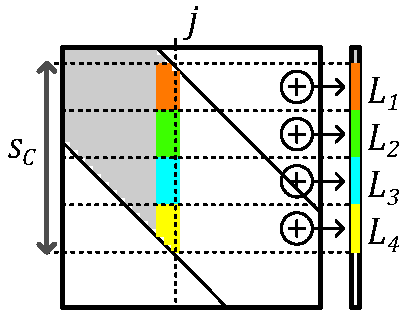
\includegraphics[width=\linewidth]{Figures/PDF/PBrotationCase1_0.pdf}
%         \caption{Column iteration $j$}
%         \label{fig:in_band_rotation_00}
%     \end{subfigure}
%     \hfill
%     \begin{subfigure}{0.49\linewidth}
%         \centering
%         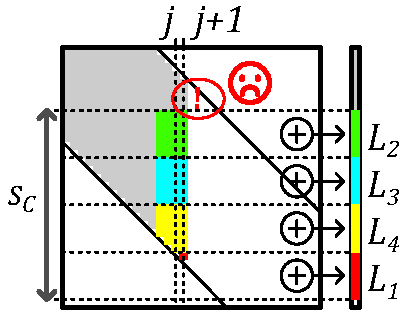
\includegraphics[width=\linewidth]{Figures/PDF/PBrotationCase1_1.pdf}
%         \caption{Column iteration $j+1$}
%         \label{fig:in_band_rotation_01}
%     \end{subfigure}
%     \caption{Example of the Eviction Rotation in a Perfect Band when the Cache is Undersized ($s_C < w_B + l - 1$)}
%     \label{fig:in_band_rotation_case1}
% \end{figure}

% \begin{figure}[htbp]
%     \centering
%     \begin{subfigure}{0.49\linewidth}
%         \centering
%         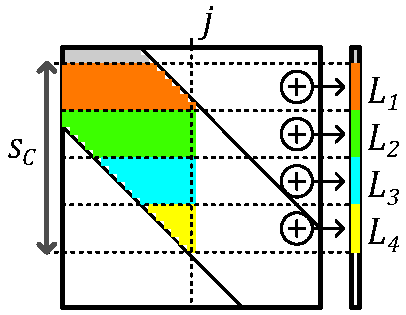
\includegraphics[width=\linewidth]{Figures/PDF/PBrotationCase2_0.pdf}
%         \caption{Column iteration $j$}
%         \label{fig:in_band_rotation_10}
%     \end{subfigure}
%     \hfill
%     \begin{subfigure}{0.49\linewidth}
%         \centering
%         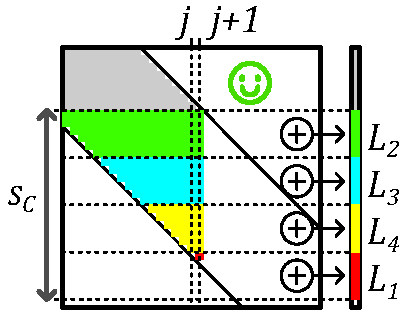
\includegraphics[width=\linewidth]{Figures/PDF/PBrotationCase2_1.pdf}
%         \caption{Column iteration $j+1$}
%         \label{fig:in_band_rotation_11}
%     \end{subfigure}
%     \caption{Example of the Eviction Rotation in a Perfect Band when the Cache is `Properly' Sized ($s_C = w_B + l - 1$)}
%     \label{fig:in_band_rotation_case2}
% \end{figure}

% We now show why the \textit{reduction cache} must be `properly' dimensioned with respect to the \textit{bandwidth} of a \textit{perfectly banded} matrix, in order to avoid unnecessary evictions when processing an \algo{OP} SpMV kernel.
% Indeed, if the cache is too small compared to the band, evictions occur before the column iteration is over, leading to poor data-reuse for the next iteration.
% To achieve high data-reuse, we show that the cache-size ($s_C$) and the \textit{bandwidth} ($w_B$) must respect the relationship given in Equation~\ref{eq:in_band_cond}.

% \begin{equation}
%     s_C \geqslant w_B + l - 1
%     \label{eq:in_band_cond}
% \end{equation}

% We consider two examples with a cache having four cache-lines ($L_1$ to $L_4$) with $l = 6$.
% In Figure~\ref{fig:in_band_rotation_case1}, we illustrate the case when the cache is too small ($s_C < w_B + 5$).
% In Figure~\ref{fig:in_band_rotation_00}, we see the state of the cache after iterating up to column $j$.
% Then, in Figure~\ref{fig:in_band_rotation_01}, we see the state after processing the next column, $j+1$.
% The cache-line $L_1$ (\textit{orange}) is evicted, and allocated to new elements at the bottom of the band, below the \textit{yellow} area.
% In this case, there are still elements of the band above the \textit{green} area, whose corresponding cache-line has, unfortunately, been evicted.
% Thus, on iteration $j+2$, cache-line $L_1$ must be fetched again and this pattern continues creating \textit{thrashing}.

% In Figure~\ref{fig:in_band_rotation_case2}, we illustrate the case when the cache is `properly' sized ($s_C \geqslant w_B + 5$).
% As in the previous example, Figures~\ref{fig:in_band_rotation_10} and~\ref{fig:in_band_rotation_11} show the state of the cache at iterations $j$ and $j+1$, respectively.
% This time, the cache-line $L_1$ is evicted only when all elements of the band in the \textit{orange} region have been processed.
% Indeed, the eviction of cache-line $L_1$ occurs just in time so that it can be allocated to the new region at the bottom of the band, below the \textit{yellow} area.
% In this way, when processing columns, the cache-lines do a rotation where the top one is evicted and allocated at the bottom, with one eviction occurring after the processing of every $l$ columns.

% If the cache-size is larger than required by Equation~\ref{eq:in_band_cond}, the rotations are the same, the eviction-rate is the same, but each cache-line accumulates more elements, increasing the hit-rate.
% To produce this perfect cache rotation, we assume an LRU eviction policy and dense vertical-strips, although, even with a \textit{random} policy, the general pattern still holds.

% This analysis shows that, with a ``properly-sized'' \textit{reduction cache}, a \textit{perfectly banded} matrix provokes no unnecessary evictions and the cache-lines are fully utilized.
% Many real matrices are banded, but are rarely \textit{perfectly banded}, and next, we study the impact of non-zero elements out of the band.

% % %%%%%%%%%%%%%%%%%%%%%%%%%%%%%%%%%%%%%%%%%%%%%%%%%%%%%%%%%%%%%%%%%%%%%
% \subsection{Impact of Out-Of-Band Density on Memory Traffic}
% \label{sec:graph1}

% We now apply the analytical model of Section~\ref{sec:redcache_model} to analyse the performance of a \textit{reduction cache} for banded matrices, processing an \algo{OP} SpMV kernel ($A \times b = c$).
% We consider banded matrices of dimension $M = 1000$, with a half-band of size $w_\mathit{hB} = 125$ and an in-band density $d_\mathit{IB} = 1$.
% We analyse a 4-way set-associative cache ($W = 4$) with a cache-line size of $l = 8$ elements, with a \textit{random} eviction policy.
% The size of the cache varies from $S = 1$ to $S = 32$ \textit{sets}.
% When the cache-size reaches $S = 32$, the cache can hold the full output vector: $S \times W \times l \geqslant M$.
% In Figure~\ref{fig:theory_traffic_vs_d_ob}, we plot the normalized memory traffic, $\mathit{normMT}$, for the output vector $c$, depending on the out-of-band density $d_\mathit{OB}$, for varying cache-sizes.

% \begin{figure}[htbp]
%     \centering
%     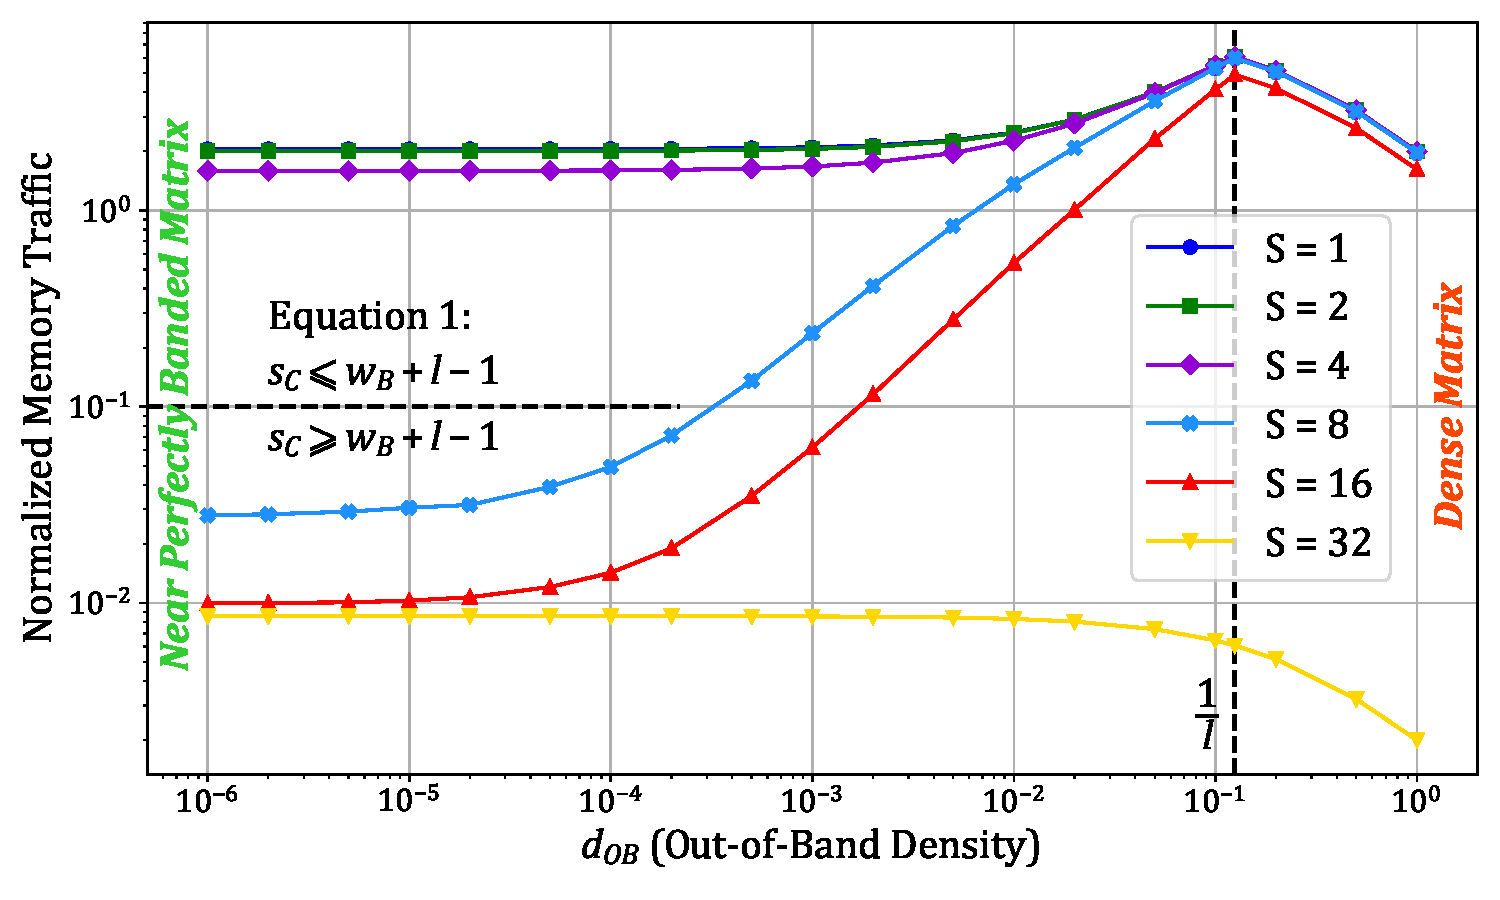
\includegraphics[width=\linewidth]{Figures/PDF/graph1_25.07.31.pdf}
%     \caption{Normalized Output Memory Traffic Depending on the Out-of-Band Density for Several Cache-Sizes}
%     \label{fig:theory_traffic_vs_d_ob}
% \end{figure}

% On the right of the graph, we notice that $\mathit{normMT}$ reaches a peak when the out-of-band density equals \mbox{$\frac{1}{l} = 0.125$}.
% Indeed, when there is at least one non-zero element per cache-line, the behavior of the cache approaches that seen for a dense matrix.
% As the density increases further, the traffic remains constant, thus $\mathit{normMT}$ drops, as seen in the graph in Figure~\ref{fig:theory_traffic_vs_d_ob}

% For the plot corresponding to $S = 32$, the cache is large enough to store the entire output vector $c$, thus, there are no evictions and $\mathit{normMT}$ is constant, corresponding to the flush traffic at the end.
% This plot gives the lower bound of memory traffic for the output vector $c$.

% The first takeaway of this graph is that variations in $d_\mathit{OB}$ heavily impact $\mathit{normMT}$.
% Isolated non-zero elements outside the band trigger misses and evictions of cache-lines corresponding to the banded region.
% Furthermore, when a cache-line is allocated for an isolated out-of-band element, most of the cache-line remains empty.
% In this case, instead of the efficient rotating pattern described in Section~\ref{sec:perfectband_vs_cache}, the cache is \textit{thrashing} with low utilisation.
% Regardless of the cache-size, the lower the out-of-band density, the lower $\mathit{normMT}$, as seen by the plots that tend downward toward the left of the graph.
% Avoiding the perturbations induced by the out-of-band elements would enable the cache to achieve minimal memory traffic, as with a \textit{perfectly banded} matrix.

% Not surprisingly, at the left of the graph, $\mathit{normMT}$ varies depending on the cache-size.
% This is due to the relative size of the band and the cache.
% Indeed, if the matrix \textit{bandwidth} is large compared to the cache-size, processing one column of the band will generate many evictions.
% To avoid evictions in the band, the relationship given by Equation~\ref{eq:in_band_cond} in Section~\ref{sec:perfectband_vs_cache} must be fulfilled.
% Indeed, for this example, for $S \geqslant 8$, this relationship holds and the corresponding plots have significantly lower $\mathit{normMT}$.
% Conversely, the first three plots ($S = 1$ to $4$) do not respect this condition, explaining their high $\mathit{normMT}$.
% Thus, the second takeaway from this graph is that, given a cache memory size, there is an ideal \textit{bandwidth} that generates minimal $\mathit{normMT}$.
% Increasing the cache-size beyond this threshold only produces a minor reduction in memory traffic, since at the beginning of matrix traversal, the first eviction is deferred before reaching the steady state rotating pattern, as discuss in Section~\ref{sec:perfectband_vs_cache}.

% These observations lead us to divide the cache into two regions.
% One which is optimized for storing the band and the other which handles all the other elements.
% The in-band region of the cache can thus operate with maximal efficiency corresponding to the bottom-left of Figure~\ref{fig:theory_traffic_vs_d_ob}.
% In subsequent sections, we analyse the out-of-band traffic.

% % %%%%%%%%%%%%%%%%%%%%%%%%%%%%%%%%%%%%%%%%%%%%%%%%%%%%%%%%%%%%%%%%%%%%%
% \subsection{Design Analysis for Out-of-Band Region}
% \label{sec:graph2}

% For the type of large matrices under study, there are usually too many non-zero elements in the out-of-band region for them to be cached from one column to the next, thus making it impossible to achieve the rotating pattern described in Section~\ref{sec:perfectband_vs_cache}.
% Therefore, the size of the cache for the out-of-band is not as important as the choice of associativity and data granularity.
% To justify this affirmation, we use the analytical model from Section~\ref{sec:redcache_model} to analyse the performance of the \textit{reduction cache} when processing only the non-zero elements outside of the band.
% As we have already discussed the handling of the in-band region, we now consider only the out-of-band elements, which is equivalent to setting the in-band density to $d_\mathit{IB} = 0$.
% Using the same matrix parameters as in the previous section, we explore different choices of cache-line size ($l \in \{1, 8\}$ elements), associativity (set-associative or fully-associative), memory transaction type (\textit{R/W} or \textit{RMW}), and total cache-size ($s_C \in \{128, 256\}$ elements).
% Because the out-of-band data is highly sparse, we want to explore having an element-wise cache ($l = 1$) instead of the typical line-wise cache ($l = 8$).
% As this cache region can be relatively small, a fully-associative configuration ($S = 1$, $l = 1$) is reasonable in terms of hardware implementation, and this full associativity makes full use of the storage.
% Indeed, when dealing with sparse elements, it is wasteful to bring a full line into the cache to only modify one element and then evict it, which we denote as \textit{R/W}.
% Thus, we consider offloading the \textit{reduction} to a higher level cache, thus reducing unnecessary data transfers.
% We assume the higher level cache can support this operation which we denote as \textit{RMW}.
% Indeed, protocols such as AXI~\cite{ARM2023_AXI} support atomic transactions (AMOs), which could easily be extended for \textit{reduction} operations.

% To validate that the cache-size is of secondary importance, we consider two different sizes (\textit{solid} and \textit{dashed}).
% For a given cache-size, we adjust the number of ways ($W$), based on the associativity, to keep the cache-size constant.
% In Figure~\ref{fig:theory_OBtraffic_vs_d_OB}, we plot $\mathit{normMT}$ for the output vector, depending on $d_\mathit{OB}$, for varying cache configurations.

% \begin{figure}[htbp]
%     \centering
%     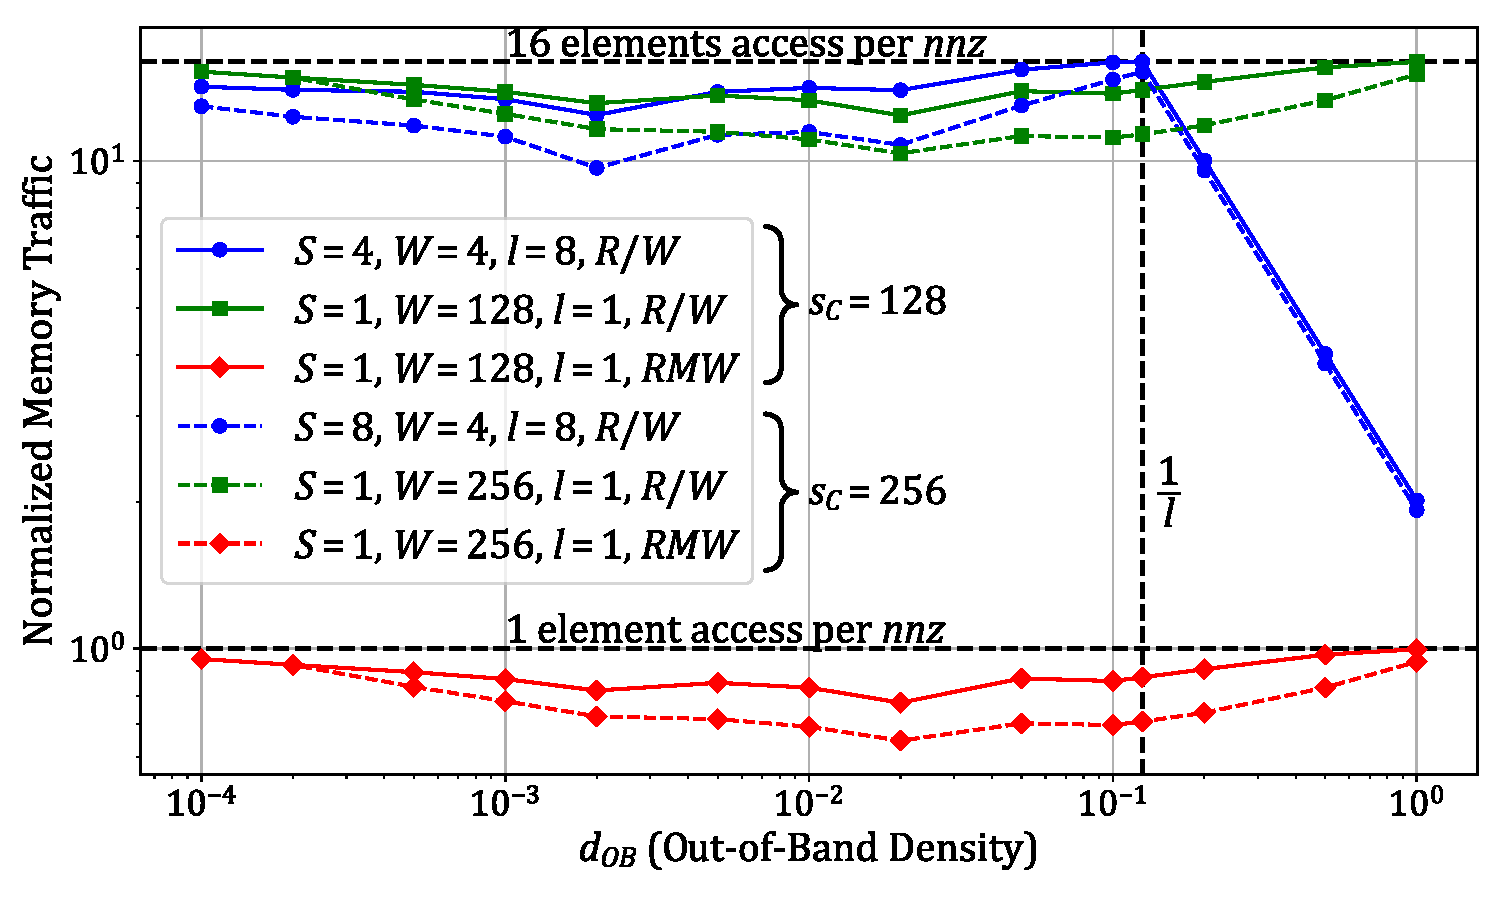
\includegraphics[width=\linewidth]{Figures/PDF/graph3_25.07.31_modif.pdf}
%     \caption{Normalized Output Memory Traffic of the Out-of-Band, Depending on the Density for Several Cache-Sizes}
%     \label{fig:theory_OBtraffic_vs_d_OB}
% \end{figure}

% Let us start by considering a classic set-associative cache with a line-wise memory interface (\textit{solid blue}, \textit{dot}), where we see a dependence of $\mathit{normMT}$ on $d_\mathit{OB}$.
% On the right of the graph ($d_\mathit{OB} \geqslant \frac{1}{l}$), we observe the same behavior as in Section~\ref{sec:graph1}, where the cache behavior approaches that seen for a dense matrix, where the cache tends to \textit{thrash}.

% Looking at the plot for the fully-associative cache with a line-wise memory interface (\textit{solid green}, \textit{square}), we see that the normalized traffic is not impacted by the density of the out-of-band, as expected.
% With the fully-associative cache, $\mathit{normMT}$ is constant near $16$, as, on average, there are two line-wise transactions per non-zero element processed, one read to fill the line, one write to evict it.

% The \textit{red} plots (\textit{diamond}) correspond to a fully-associative cache with an element-wise memory interface, which can offload element-wise \textit{RMW} transactions.
% We see that this approach results in over an order magnitude reduction in $\mathit{normMT}$.
% First, we avoid transferring full cache-lines which are mostly empty, and we only send the \textit{RMW} in one direction (``fire-and-forget'').
% Indeed, $\mathit{normMT}$ is now reduced to below one transaction per non-zero element processed.
% The fact that this value is below one shows that this cache region does hit and reduce memory traffic.
% However, increasing the size of this cache does not significantly increase the hit-rate, as can be seen by the \textit{dashed} plots, which correspond to a $2\times$ larger cache, and which are not significantly lower than the corresponding \textit{solid} ones.

% To summarize, the characteristics needed for the out-of-band region are: (1) a fully-associative element-wise data-storage to avoid virtually empty cache-lines, (2) an element-wise memory interface to reduce memory traffic, and (3) a small storage region which is adequate.

% % %%%%%%%%%%%%%%%%%%%%%%%%%%%%%%%%%%%%%%%%%%%%%%%%%%%%%%%%%%%%%%%%%%%%%
% \subsection{Resulting Approach and Discussion}
% \label{sec:theory_conclu}

% In the previous sections, we analyzed the behavior of \textit{reduction caches} executing an \algo{OP} SpMV kernel with banded matrices.
% We evaluated the expected memory traffic using an analytical model, considering separately the in- and out-of-band regions.
% We identified the cache characteristics required for both regions, which are extremely different.
% We thus propose to divide the available cache memory into two dedicated regions: one for the in-band, and one for the out-of-band.

% To obtain the efficient rotating pattern for the in-band region, which is the key to massively reducing memory traffic, Equation~\ref{eq:in_band_cond} must be respected.
% In practice, this defines the size of the band that can be allocated to the in-band cache region.
% As we have seen, this cache region can operate efficiently with a set-associative line-wise configuration.

% For the out-of-band region, a fully-associative element-wise cache with an element-wise memory interface can significantly reduce the memory traffic.
% The size of this region is less critical, thus it is preferable to allocate the majority of the available storage to the in-band region.

% It is important to note that the analytical model that we have presented is based on the assumption of a uniform distribution of the non-zero elements.
% In practice, this is not always the case, and this non-uniformity can impact the cache behavior, as will be seen later in Section~\ref{sec:evaluation}.
% Indeed, if the non-zero elements are clumped, the cache-lines tend to be better filled, resulting in lower memory traffic.
% In other words, our uniform assumption leads to a pessimistic prediction of memory traffic.

\clearpage